\documentclass{article}
\usepackage{graphicx} % Required for inserting images
\usepackage{hyperref}
\usepackage{gensymb}
\usepackage{amsmath}
\usepackage{tfrupee} 
\title{Algebra }
\author{AKSHAY KUMAR}
\date{August 2023}
\graphicspath{{/sdcard/fwc/latex/figs}}
\begin{document}

\maketitle

                     {SECTION A}
\begin{enumerate}
    \item If $\sin \theta=0$ then the value of $\tan^2\theta$+$\cot^2\theta$ is
    \begin{enumerate}
        \item 2  \item 4
        \item 1
        \item $\frac{10}{9}$
    \end{enumerate}
    \item The value(s) of k for which the quadratic equation $3x^2-kx+3=0$ has
equal roots, is (are) 
\begin{enumerate}
    \item 6 
    \item -6
    \item +-6
    \item 9
\end{enumerate}
\item $5tan^2 \theta-5sec^2\theta= \underline{\hspace{2cm}}$

 \item If$\alpha$,$\beta$ are zeroes of the polynomial $2x^2-5x-4 $then$\frac{1}{\alpha}+\frac{1}{\beta}$
     \item In Figure\ref{as.jpg},a tower stands vertically on the ground.From a point on the ground,which is 80m away from the foot of the tower,the angle of elevation of the tower is found to be 30\degree Find the height of the tower
\begin{figure}[htbp]
    \centering
    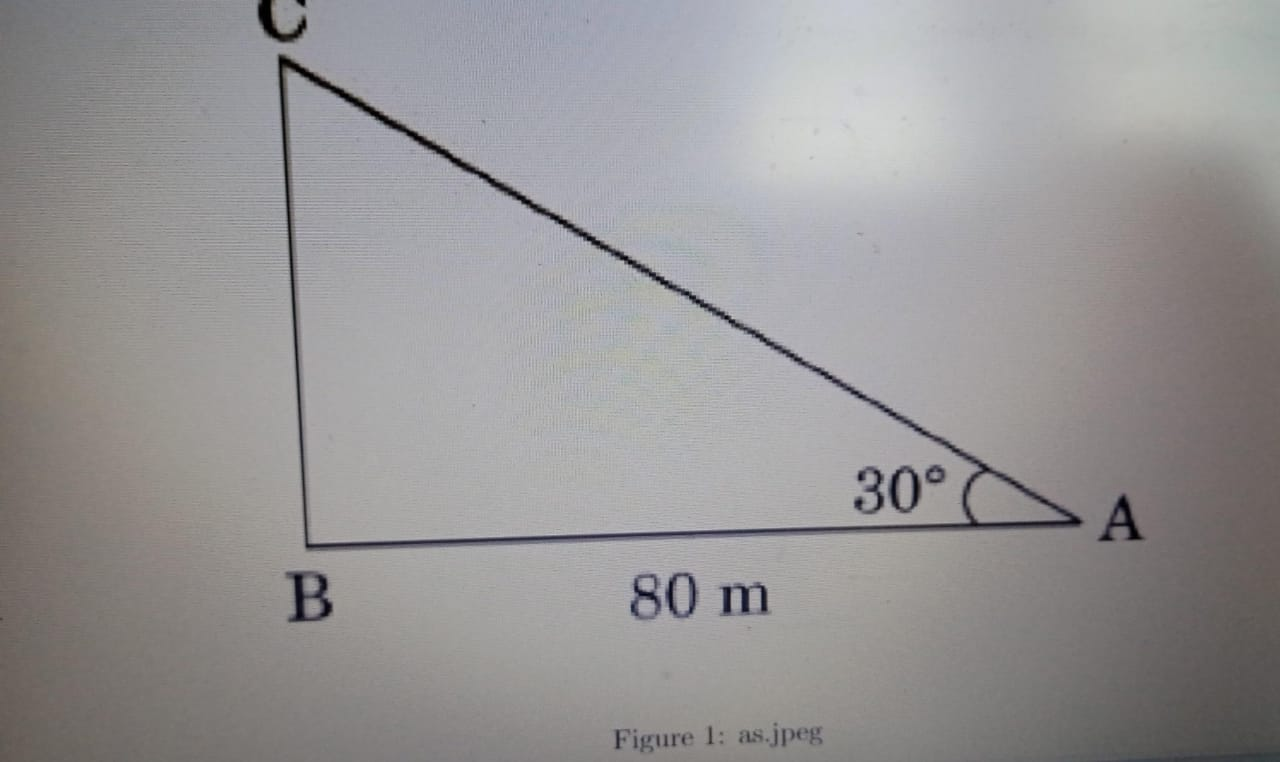
\includegraphics[width=\columnwidth]{figs/as.jpeg}
    \caption{as.jpeg}
    {\label{as.jpg}}
\end{figure}

\item Solve $9x^2-6a^2x+a^4-b^4$ using quadratic formula.

\item Show that $\cos(38\degree) \cos(52\degree)-\sin(38\degree)\sin(52\degree)=\cos(90\degree)$.
\item Prove that 
\begin{align}
\frac{sin\theta}{cot\theta+csc\theta}=2+\frac{sin\theta}{cot\theta-csc\theta}.
\end{align}
\item given 15$\cot (A)$=8,find the values of $\sin (A)$and $\sec (A)$.
\item The angles of depression of the top and bottom of a tower as seen from the top of a $60\sqrt{3}m$ high cliff are $45\degree$ and $60\degree$ respectively. Find the height of the tower.(Use $\sqrt{3}=1.73$)
\item A and B jointly finish a piece of work in 15 days. When they work 
separately, A takes 16 days less than the number of days taken by B to 
finish the same piece of work. Find the number of days taken by B to 
finish the work.
\item If the polynomial \begin{align} 
f(x)=3x^4-9x^3+x^2+15x+k
\end{align} is completely divisible by $3x^2-5$,then find the value of $k$.Using the quotient, so obtained, find two zeroes of the 
\item Find all the zeroes of the polynomial \begin{align}
    f(x)x^4-8x^3+23x^2-28x+12
\end{align} if two of its zeroes are 2 and 3.  
    \item Find the value of m for which the quadratic equation
    \begin{align}
                      (m-1)x^2+2(m-1)x+1=0
                  \end{align} has two real and equal roots. 
                  \item Solve the following quadratic equation for x 
                  \begin{align}
                      \sqrt{3}X^2+10x+7\sqrt{3}=0
                  \end{align}
                  \item  The product of Rehan's age(in years) 5 years ago and his age 7 years from now, is one more than twice his age. Find his present age.
                  \item The angle of elevation of the top of a building from the foot of the tower is $30\degree$and the angle of elevation of the top of the tower from the foot of the building is $60\degree$. If the tower is $50\degree$ m high, then find the height of the building.
                 \item From a point on a bridge across a river, the angles of depression of the banks on opposite sides of the river are $30\degree$ and $60\degree$respectively. If the bridge is at a height of 3 m from the banks, then find the width of the river 
                 \item In figure\ref{ak.jpg} Gadisar Lake is located in the Jaisalmer district of Rajasthan. It was built by the King of Jaisalmer and rebuilt by Gadsi Singh in 14th century. The lake has many Chatris. One of them is shown below
\begin{figure}[htbp]
\centering
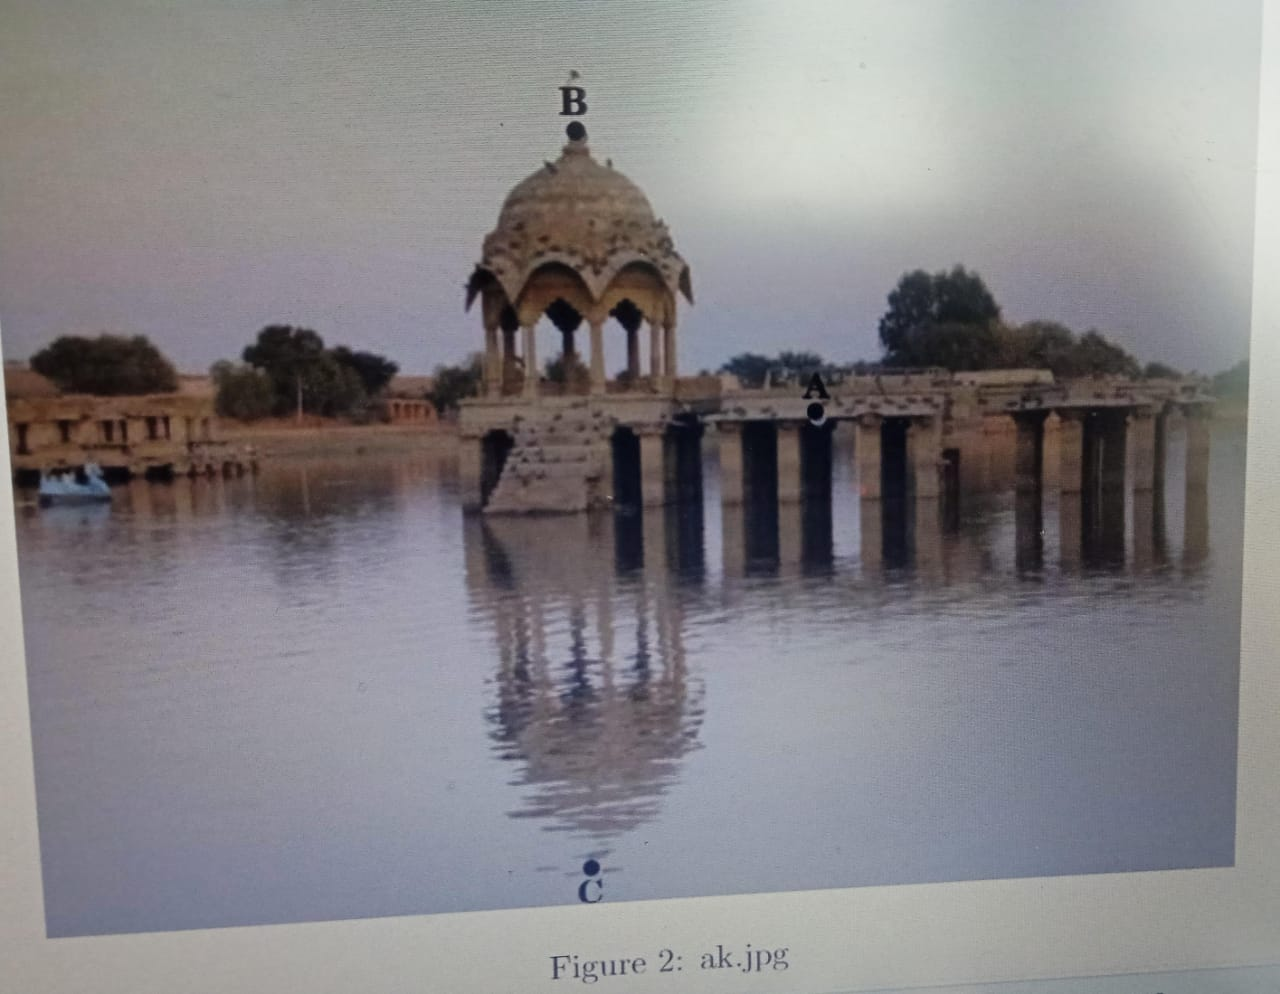
\includegraphics[width=\columnwidth]{figs/ak.jpg}
\caption{ak.jpg}
\label{ak.jpg}
\end{figure}.
Observe the picture. From a point A h m above from water level, the 
angle of elevation of top of Chhatri (point B) is $45\degree$and angle of 
depression of its reflection in water (point C) is $60\degree$ . If the height of 
Chhatri above water level is (approximately) 10m, then 
\begin{enumerate}
\item draw a well-labelled figure based on the above information
\item find the height(h) of the point $A$ above water level.(Use$\sqrt{3}=1·73$) 
\end{enumerate}
       \item solve the quadratic equation 
       $x^+2\sqrt{2x}-6=0$ for x
       \item In figure\ref{su.jpg} From put on bridge across a river, the angles of depression of the banks on opposite sides of the river are $30\degree$ and $45\degree$. If the bridge in at a height of 8 m from the banks, then find the width of the river.
       \begin{figure}[htbp]
\centering
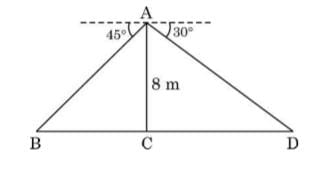
\includegraphics[width=\columnwidth]{figs/su.jpg}
\caption{su.jpg}
\label{su.jpg}
\end{figure}.
\item A 2-digit number is such that the product of it digits is 24. If 18 is subtracted from the number, the digits interchange their places. Find the number.
       \item The difference of the squares of two numbers in 180. The square of the smaller number is 8 times the greater number. Find the two numbers.
       \item Case Study-1

$Kite Festival$
Kite festival is celebrated in many countries at different times of the year.In India, every your 14th January in celebrated as International Kite Day On this day many people visit India and participate in the festival be flying various kinds of kits
The picture given below, the kites flying together.
\begin{figure}[!h]
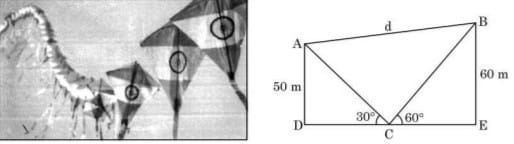
\includegraphics[width=1.0\textwidth]{figs/kite.jpg}
\caption{kites}
\label{kite.jpg}
\end{figure}     

In Fig. 5, the angles of elevation of two kites (Point A and B) from the hands of a man (Point C)are found to be $30\degree$ and $60\degree$ respectively.Taking ||AD = 50m and BE= 60m,find
\begin{enumerate}
    \item the lengths of strings used (take them straight) for kites A and B as shown in the figure
    \item the distance 'd' between these two kites
    \end{enumerate}
    \item Solve the quadratic equation for x:
    \begin{align}
    x^2-2ax-(4b^2-a^2)=0
         \end{align}
    $x^2-2ax-(4b^2-a^2)=0$
    \item If the quadratic equation
    \begin{align}
        (1+a^2)x^2+2abx+(b^2-c^2)=0
    \end{align}has equal and real roots, then prove that : 
    $b^2=c^2(1+a^2)$
\item Two boats are sailing in the sea 80 m apart from each other towards a cliff AB.The angles of depression of the boats from the top of the cliff are $30\degree$ and $30\degree$ respectively,as shown in\figureautorefname{fig5}.
Find the height of the cliff.
\begin{figure} 
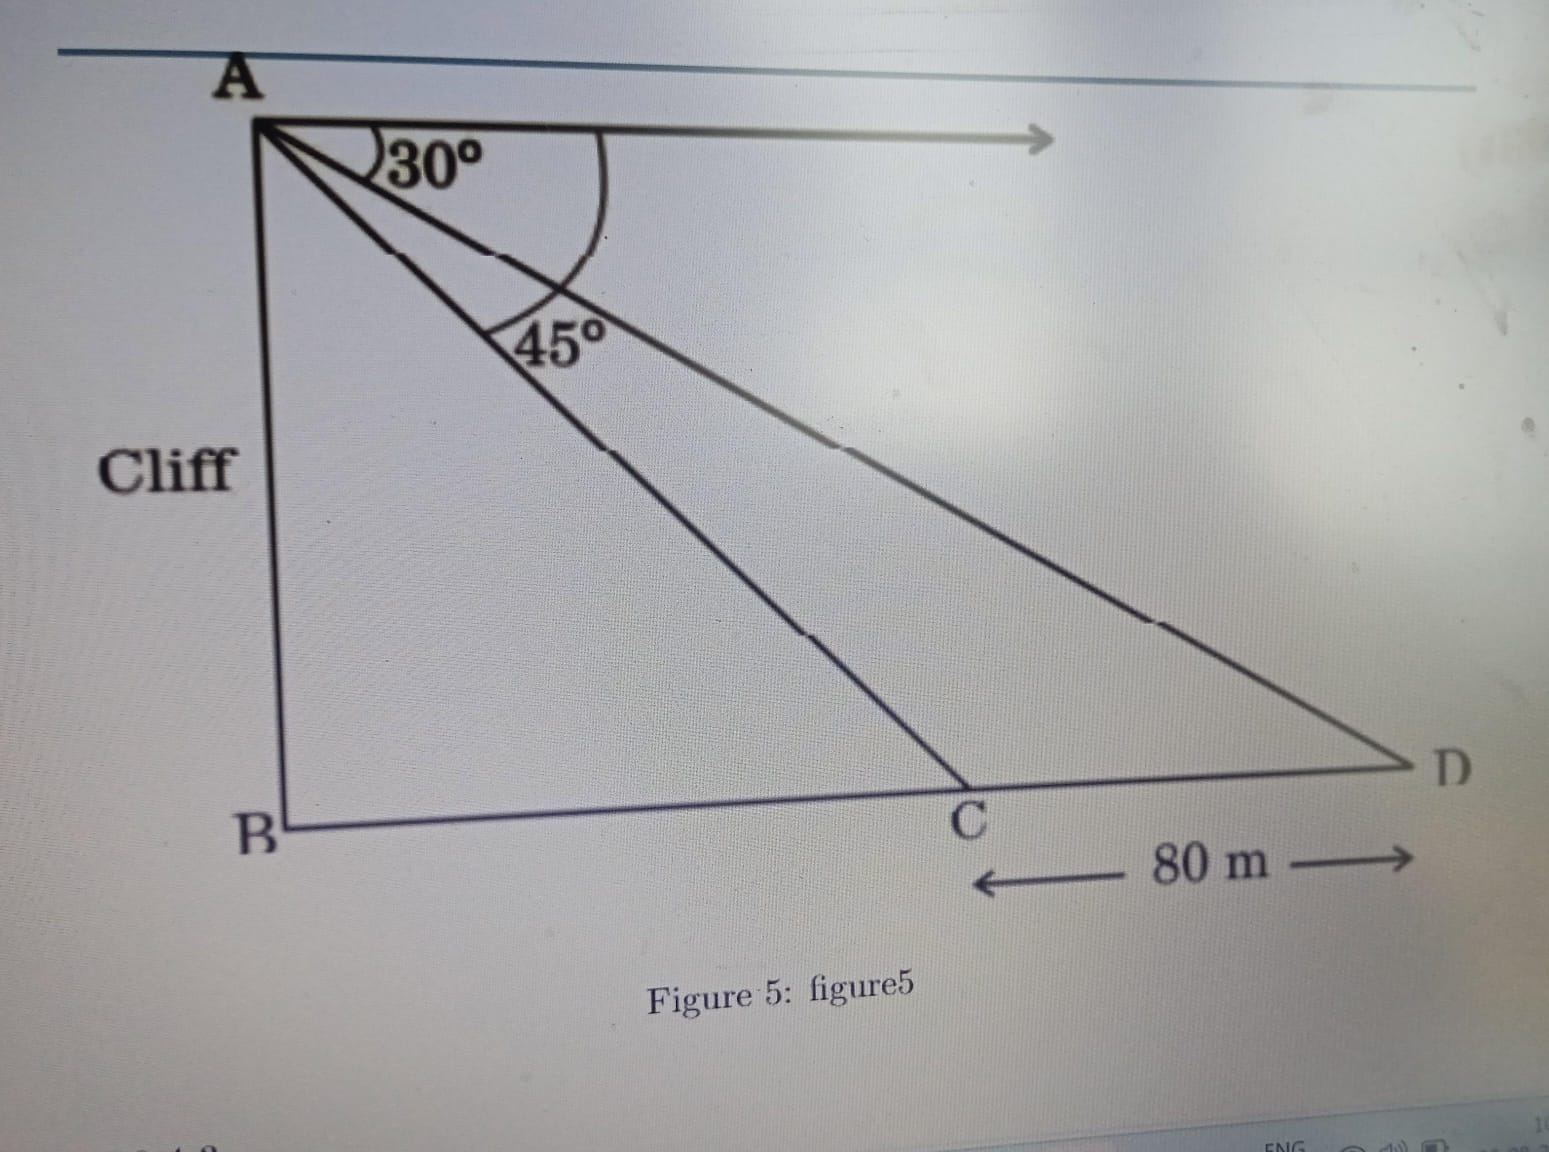
\includegraphics[width=1.1\columnwidth]{figs/boat.edit.png}
\caption{figure5}
\label{fig5}
\end{figure}
 \item The angle of elevation of the top Q of a vertical tower PQ from a point X on the ground is $30\degree$.From a point Y,40 m vertically above X, the angle of elevation of the top Q of tower PQ is $45\degree$ . Find the height of the tower PQ and the distance PX. [Use $\sqrt{3}$= 1·73] 
 \item Find the value of 'k'for which the quadratic equation 
     \begin{align}
         2kx^2-40+25=0
     \end{align} has real and equal roots.
     \item solve for x:$\frac{5}{2}x^2+\frac{2}{5}=1-2x$
     \item An aeroplane at an altitude of 200 metres observes the angles of depression of opposite points on the two banks of a river to be $45\degree$ and $60\degree$ .Find the width of the river. (Use$\sqrt{3}$ = 1.732)
     \item find the value of 'p' for which the quadratic equation $(px-4) (x-2)$
     \item Had Aarush scored 8 more marks in a Mathematics test, out of 35 marks, 7 times these marks would have been 4 less than square of his actual marks, How many marks did he get in the test?
     \item From the top of an 8 m high building, the angle of elevation of the top of a cable tower is $60\degree$ and the angle of depression of its foot is $45\degree$  . Determine the height of the tower. (Take $\sqrt{3} = 1.732$).
     \item Find the roots of the quadratic equation 
     \begin{align}
         9x^2-6\sqrt{2}x+2=0
         \end{align}
         \item The product of two consecutive odd positive integers is 255. Find the integers, by formulating a quadratic equation.
         \item Find the value(s) of k for the quadratic equation,
         \begin{align}
             (k+3)x^2+kx+1=0 
         \end{align} , to have two real and equal roots.
         \item As observed from the top of a lighthouse 60 m high from the sea level, the angles of depression of two ships are $45\degree$ and $60\degree$ . If one ship is exactly behind the other on the same side of the lighthouse, then find the distance between the two ships. [Use$\sqrt{3}$= 1·732]
         \item At a point on the level ground, the angle of elevation of the top of a vertical tower is found to be $\alpha$,such that tan$\alpha$=$\frac{5}{12}$.On walking 192 m towards the tower, the angle of elevation $\beta$ is such that tan$\beta$=$\frac{3}{4}$.Find the height of the tower. 
     \item $\tan^{-1}$ $\frac{1}{\sqrt{3}}$ - $\cot^{-1}$$\frac{-1}{\sqrt{3}}$
     \item Show that the relation R in the set R of all real numbers,defined R= $\{(a,b):a\leq b^2\}$
         \item Two angles of a triangle are $\cot^{-1}$ 2 and $\cot^{-1}$ 3.The third angle of the triangle is $?$
         \item Solve for x:
         \begin{align}
          \sin^{-1}(1-x)-2 \sin^{-1} x=\frac{\pi}{2} 
         \end{align}
\item Find the present value of a perpetuity of \rupee~18,000 at the end of 6 months is worth 8$\%$ p.a.compounded semi-annually.
\item Find the effective rate which is equivalent to nominal rate of 10$\%$ p.a.compounded monthly.

    [given that:$1.00833^{12} = 1.1047$]
    \item Abhay bought a mobile phone for\rupee~30,000. The mobile phone is estimated to have a scrap value of \rupee~3,000 after a span of 3 years. Using the linear depreciation method, find the book value of the mobile phone at the end of 2 years.    
\item Madhu exchanged her old car valued at \rupee~1,50,0000 with a new one priced at  \rupee~65,000.she paid \rupee~x as down payment and the balance in 20 monthly equal instalments of \rupee~21,000 The rate of interest offered to her is 9$\%$ p.a.Find the value of x.
    [Given that:$1.0075^{-20} = 0·86118985$] 
    \item Calculate the EMI under 'Flat Rate System' for a loan if 
\rupee~5,00,000 with 10$\%$ annual interest rate for 5 years.  
\item A machine costing \rupee~2,00,000 has effective life of 7 years and its scrap value is \rupee~30,000. What amount should the company put into a sinking fund earning 5 $\%$ p.a., so that it can replace the machine after its usual life ? Assume that a new machine will cost \rupee~3,00,000 after 7 years. 
[Given that:(1.05)$^7$ = 1.407]
\item A start-up company invested \rupee~3,00,000 in shares for 5 years. The value of this investment was \rupee~3,50,000 at the end of second year,\rupee~3,80,000 at the end of third year and on maturity, the final value stood at \rupee~ 4,50,000. Calculate the Compound Annual Growth Rate (CAGR) on the investment
[Given that:(1.5)$^\frac{1}{5}$ = 1.084 ]

     \end{enumerate}
\end{document}
